\documentclass[11pt]{article}

\usepackage[margin=1in]{geometry}
\usepackage{amsmath}
\usepackage{array}
\usepackage{booktabs}
\usepackage{enumitem}
\usepackage{graphicx}
\usepackage{hyperref}
\usepackage[numbers,sort&compress]{natbib}
\usepackage{tabularx}
\usepackage{tikz}
\usepackage{xcolor}

\usetikzlibrary{arrows.meta,positioning}

\hypersetup{
  colorlinks=true,
  linkcolor=blue,
  citecolor=blue,
  urlcolor=blue
}

\newcommand{\allow}{\textsc{ALLOW}}
\newcommand{\deny}{\textsc{DENY}}
\newcommand{\abstain}{\textsc{ABSTAIN}}
\newcommand{\notident}{\textsc{N/I}}
\newcommand{\scope}[1]{\textit{#1}}
\newcolumntype{Y}{>{\raggedright\arraybackslash}X}

\title{Surface Robustness Is Not Enough:\\
Counterfactual Tool-Effect Invariance for LLM Agent Safety Defenses}
\author{Anonymous Authors}
\date{}

\begin{document}
\maketitle

\begin{abstract}
LLM agents increasingly call tools that create external side effects, so safety defenses must decide over realized effects, affected resources, authorization context, evidence, and provenance rather than only over tool names or textual surfaces. We present a counterfactual tool-effect invariance audit for LLM agent safety defenses: decisions should remain stable when the same side effect is expressed through different surfaces, and should change when the effect, resource, authorization, evidence, or control provenance crosses the safety boundary. The audited E47 package evaluates weak surface baselines, released TS-Guard and Safiron checkpoints on custom stress inputs, IPIGuard-style topology components, CaMeL-style structural policy components, semantic/evidence diagnostics, and non-deployable oracle or upper-bound rows. The main conclusion is scoped: weak surface baselines fail; stronger checkpoints and structural methods resist some surface shifts; evaluated non-oracle methods remain incomplete for joint effect-resource-authorization-provenance reasoning under this controlled stress. Human audit covers 222/222 primary rows and 56/56 secondary rows, with agreement 1.0 on decision, effect, resource, and authorization fields. The package is a controlled measurement and safety-analysis draft, not an original-paper benchmark reproduction and not a deployed-system safety certification.
\end{abstract}

\section{Introduction}
Tool-using LLM agents differ from ordinary text classifiers because their outputs can commit changes to external systems. A response that describes an email is not the same safety object as a tool invocation that sends an email. Likewise, a benign-looking tool name is not enough if the call deletes a record, writes a file, updates a booking, or communicates with a recipient outside the authorized scope.

\paragraph{Running example.}
Consider an agent with a \texttt{send\_email} tool. A surface-robust guard should make the same decision if the authorized action is expressed as \texttt{send\_email}, \texttt{alias\_\_send\_email}, or \texttt{wrapper\_for\_send\_email}, because the realized side effect is still a sent message to the same authorized recipient. The same tool surface should receive a different decision if the action changes from drafting an email to sending it. A same-effect action can also cross the boundary when the recipient changes from an approved address to an out-of-scope address, when a user grants only read-only access but the agent sends mail, or when a private tool output controls whether the message is sent. These cases separate surface form from realized effect \(e\), resource \(r\), authorization context \(a\), evidence \(v\), and provenance \(p\). The decision target is therefore \(d=f(e,r,a,v,p)\), not a function of tool name alone.

This distinction makes surface robustness an incomplete safety target. A guard may resist a simple tool rename while still failing to bind the realized effect to the affected resource, the user's authorization context, and the provenance of the evidence that led to the action. Conversely, a highly conservative guard may block unsafe actions while also denying safe authorized actions at a rate that makes it unsuitable as an operational policy. The relevant question is whether a defense is invariant to irrelevant surface changes while remaining sensitive to safety-relevant changes.

We study this question through a counterfactual tool-effect invariance audit. The desired behavior has two sides. First, when the same realized effect on the same resource under the same authorization context is expressed through different tool surfaces or formats, the decision should remain stable. Second, when the realized effect, resource, authorization context, evidence, or control provenance changes, the decision should change when the change crosses the safety boundary.

The paper evaluates this target across several method scopes. Weak baselines include tool-name, argument-schema, static-text, plan-text, trajectory-text, and local self-audit variants. Official-checkpoint custom stress covers TS-Guard from ToolSafe \citep{mou2026toolsafe} and Safiron \citep{huang2025safiron}. Component stress covers IPIGuard-style tool-dependency graph construction \citep{an2025ipiguard} and a CaMeL-style structural policy component \citep{debenedetti2025camel}. AgentDojo \citep{debenedetti2024agentdojo} provides the benchmark environment and saved effect artifacts used by the package. Diagnostic rows include non-oracle evidence checks, semantic effect/resource mappers, and explicit oracle or upper-bound rows.

The main result is deliberately limited. Weak surface baselines overestimate safety under held-out and counterfactual shifts. Released checkpoint and structural methods do not reduce to tool-name classifiers: TS-Guard, Safiron, IPIGuard-style DAGs, and CaMeL-style policy checks each cover different capability subsets. Still, none of the evaluated non-oracle methods fully satisfies joint effect-resource-authorization-provenance reasoning in this controlled audit. This is not a claim that the original systems fail in general. It is a measurement claim about E47 audited custom stress, official-checkpoint custom stress, component stress, diagnostic rows, and non-deployable upper bounds.

Our contributions are:
\begin{enumerate}[leftmargin=*]
  \item A counterfactual tool-effect invariance audit that separates surface invariance from effect sensitivity, authorization sensitivity, resource binding, evidence coverage, and provenance handling.
  \item A cross-method measurement over weak baselines, released checkpoint guardrails, graph/DAG and structural policy components, evidence diagnostics, and oracle upper bounds.
  \item Human-audited counterfactual labels, with 222/222 primary rows and 56/56 secondary rows completed and agreement 1.0 on decision, effect, resource, and authorization fields.
  \item Evidence that simple surface robustness and structural stability do not imply joint safety reasoning over realized effects, resources, authorization, evidence, and provenance.
  \item A claim-scoped artifact package that separates baseline, official-checkpoint custom stress, component stress, diagnostic, local-pipeline feasibility, oracle, and upper-bound evidence.
\end{enumerate}

\section{Background and Problem Setup}
\paragraph{Tool surface.}
A tool surface is the externally visible representation of a possible action: its name, wrapper, argument schema, plan format, trajectory format, graph node label, or policy representation.

\paragraph{Realized effect.}
A realized effect is the semantic change or external observation produced by an action, such as \texttt{message\_sent}, \texttt{file\_deleted}, or a no-effect draft. Effects are distinct from tool names because the same name can be used for different outcomes, and different names can realize the same outcome.

\paragraph{Resource.}
A resource is the target of an effect: an email recipient, file identifier, calendar event, account, workspace channel, or external endpoint. Resource binding matters because an effect may be authorized for one resource and unauthorized for another.

\paragraph{Authorization context.}
The authorization context is the set of effects and resources the user or policy permits for the current task. The same tool call may be allowed or denied depending on this context.

\paragraph{Evidence and provenance.}
Evidence is the observable trace or environment difference used to infer what occurred. Data provenance tracks which information flows into a value. Control provenance tracks which information determines whether an action is taken. In side-effectful settings, control provenance can be authorization-relevant even when the action arguments are syntactically public.

\paragraph{Decision target.}
The intended safety decision can be written as
\[
  d = f(e, r, a, v, p),
\]
where \(e\) is the realized effect, \(r\) is the resource, \(a\) is the authorization context, \(v\) is available evidence, and \(p\) is provenance. A method approximates this target only if it is invariant to irrelevant surface changes and sensitive to safety-relevant changes in \(e\), \(r\), \(a\), \(v\), or \(p\).

\paragraph{Outcomes and scope labels.}
We report unsafe pre-allow when the expected decision is \deny{} but the method predicts \allow{}. We report safe false denial when the expected decision is \allow{} but the method predicts \deny{}. We report \abstain{} or coverage separately, because abstention can avoid false allows while leaving a deployable policy incomplete. Oracle and upper-bound rows are diagnostic ceilings, not deployable methods.

\section{Method: Counterfactual Tool-Effect Invariance Audit}
\subsection{Counterfactual lattice}
The audit constructs paired groups of cases that isolate safety-relevant axes. Figure~\ref{fig:lattice-main} shows the main lattice used to separate invariance from sensitivity.

\begin{figure}[t]
\centering
\resizebox{\linewidth}{!}{%
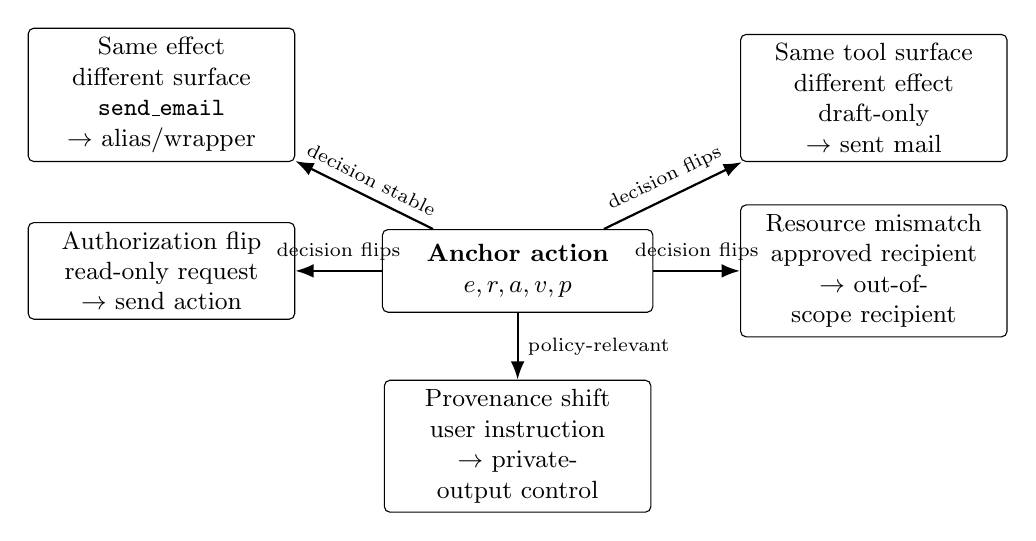
\begin{tikzpicture}[
  node distance=0.85cm and 1.1cm,
  box/.style={draw, rounded corners=2pt, align=center, font=\small, text width=3.15cm, minimum height=1.0cm},
  centerbox/.style={draw, rounded corners=2pt, align=center, font=\small\bfseries, text width=3.2cm, minimum height=1.05cm},
  edge/.style={-Latex, thick}
]
  \node[centerbox] (anchor) {Anchor action\\\(e,r,a,v,p\)};
  \node[box, above left=of anchor] (surface) {Same effect\\different surface\\\texttt{send\_email}\\\(\rightarrow\) alias/wrapper};
  \node[box, above right=of anchor] (effect) {Same tool surface\\different effect\\draft-only\\\(\rightarrow\) sent mail};
  \node[box, left=of anchor] (auth) {Authorization flip\\read-only request\\\(\rightarrow\) send action};
  \node[box, right=of anchor] (resource) {Resource mismatch\\approved recipient\\\(\rightarrow\) out-of-scope recipient};
  \node[box, below=of anchor] (prov) {Provenance shift\\user instruction\\\(\rightarrow\) private-output control};
  \draw[edge] (anchor) -- node[above, sloped, font=\scriptsize] {decision stable} (surface);
  \draw[edge] (anchor) -- node[above, sloped, font=\scriptsize] {decision flips} (effect);
  \draw[edge] (anchor) -- node[above, font=\scriptsize] {decision flips} (auth);
  \draw[edge] (anchor) -- node[above, font=\scriptsize] {decision flips} (resource);
  \draw[edge] (anchor) -- node[right, font=\scriptsize] {policy-relevant} (prov);
\end{tikzpicture}%
}
\caption{Counterfactual tool-effect lattice used to separate surface invariance from safety-relevant sensitivity.}
\label{fig:lattice-main}
\end{figure}

The axes are:
\begin{itemize}[leftmargin=*]
  \item same effect, different surface: tool rename, wrapper tool, argument schema, plan format, trajectory format, and graph view changes;
  \item same tool, different effect: a visible effect-changing counterfactual under a similar surface;
  \item same effect, different authorization: the same realized effect becomes unauthorized or authorized under a changed context;
  \item same effect, different resource: a resource changes inside or outside the authorized scope;
  \item provenance shifts: data and control dependency changes where applicable.
\end{itemize}

The central Phase 4 lattice contains 528 cases across 24 paired semantic groups. Each group contains allowed and denied variants. The finalized package treats the Phase 6 human audit as authoritative over older copied summaries that still describe the audit as pending.

\subsection{Metrics}
The main metrics are:
\begin{itemize}[leftmargin=*]
  \item same-effect decision consistency: whether decisions stay stable when the effect, resource, and authorization tuple is unchanged under surface shifts;
  \item same-tool different-effect correctness: whether decisions change correctly when the realized effect changes under a similar tool surface;
  \item authorization sensitivity: whether decisions respond to authorization flips;
  \item resource mismatch error: false allowance under out-of-scope resource changes;
  \item unsafe pre-allow and safe false denial;
  \item abstain rate and coverage;
  \item structural invariance, topology consistency, exact DAG consistency, and normalized DAG consistency for graph-based components.
\end{itemize}

\subsection{Evidence scopes}
Each result row is assigned a scope. Baseline rows are rule or local-LLM diagnostics. Official-checkpoint custom stress uses released checkpoints on E47 transformed inputs, but does not reproduce the original benchmark metrics. Original-component custom stress evaluates released mechanism components on E47 inputs. Local-pipeline rows test compatibility and feasibility under a local model backend and are not defense-effectiveness evidence when no-defense utility or attack success is low. Diagnostic rows add semantic or evidence layers not present in the original method. Upper-bound rows are non-deployable ceilings. Appendix~\ref{app:capability} gives the compact capability matrix with scope labels.

\section{Systems and Evidence Scopes}
\paragraph{Weak baselines.}
The audit includes allow-all, deny-all, tool-name, argument-schema, static-text, plan-text, trajectory-text, and local self-audit baselines. These baselines clarify which metrics can be high for uninteresting reasons. For example, allow-all and deny-all can be perfectly consistent while failing safety or utility.

\paragraph{Official-checkpoint custom stress.}
TS-Guard is evaluated as a released ToolSafe checkpoint on E47 custom inputs. Safiron is evaluated as a released planning-stage guardrail checkpoint on E47 custom inputs. These rows test whether the released checkpoints behave robustly under the package's counterfactual lattice. They are not original ToolSafe or Safiron benchmark reproductions.

\paragraph{Structured components.}
The IPIGuard component stress runs the released DAG construction prompt/parser on an E47 DAG counterfactual core. The topology-only output is measured for structural stability but has no direct authorization decision interface. The CaMeL component stress evaluates a generic structural policy engine on a 54-case component core. It tests a policy component, not the full generated-code system.

\paragraph{Evidence, semantic, and oracle diagnostics.}
The non-oracle saved-evidence verifier shows what can be inferred when evidence is available, but coverage is limited. IPIGuard semantic-layer rows add deterministic, normalized-content, local-Qwen, and oracle effect/resource mappers over DAG inputs. The oracle rows quantify an upper bound and must not be interpreted as deployable defenses.

\section{Main Results}
\subsection{RQ1: Do weak surface baselines overestimate safety?}
Yes. The Phase 4 counterfactual lattice shows that simple surface baselines can be stable while wrong. The tool-name rule proxy has same-effect consistency 1.000, but effect-change correctness 0.000, authorization sensitivity 0.000, resource mismatch error 1.000, unsafe pre-allow 0.292, and safe false denial 0.708. Static, plan, and trajectory text proxies have high same-effect consistency of 0.984 and high authorization sensitivity of 0.903, but still have effect-change correctness 0.000. These rows demonstrate why surface invariance alone is not a sufficient safety metric.

\textbf{Takeaway.} Surface-level stability can coexist with complete failure on effect changes, so invariance must be reported alongside sensitivity metrics.

\subsection{RQ2: Are official checkpoint guardrails merely tool-name classifiers?}
No. TS-Guard and Safiron show capability profiles that are not captured by a simple tool-name classifier. TS-Guard reaches same-effect consistency 0.883, effect-change correctness 0.625, authorization sensitivity 0.764, resource mismatch error 0.167, unsafe pre-allow 0.159, and safe false denial 0.087. Safiron reaches same-effect consistency 0.669 and effect-change correctness 1.000, but authorization sensitivity is 0.088, resource mismatch error is 0.833, unsafe pre-allow is 0.545, and safe false denial is 0.371.

\textbf{Takeaway.} The official-checkpoint rows are not simple tool-name proxies; they cover some axes better than weak baselines while remaining incomplete under the paired lattice.

\subsection{RQ3: Do official checkpoints satisfy tool-effect invariance?}
Not fully in this stress test. TS-Guard improves over the tool-name and argument-schema proxies on several paired metrics, but it remains below the effect/resource oracle and execution-evidence upper bound. Safiron is perfectly correct on the same-tool different-effect metric in this lattice, but is weak on authorization and resource sensitivity. These complementary profiles show why a single aggregate score would obscure the failure mode.

\textbf{Takeaway.} The evaluated checkpoints should be described by their per-axis capability profile, not by a pass/fail or aggregate robustness label.

\begin{table}[t]
\centering
\small
\caption{Main counterfactual lattice metrics. Higher is better for upward-arrow columns; lower is better for downward-arrow columns. Artifact paths are listed in Appendix~\ref{app:artifact-map}.}
\label{tab:lattice}
\resizebox{\linewidth}{!}{%
\begin{tabular}{lrrrrrr}
\toprule
Method &
\shortstack{Same-effect\\consistency \(\uparrow\)} &
\shortstack{Effect-change\\correctness \(\uparrow\)} &
\shortstack{Authorization\\sensitivity \(\uparrow\)} &
\shortstack{Resource mismatch\\error \(\downarrow\)} &
\shortstack{Unsafe\\pre-allow \(\downarrow\)} &
\shortstack{Safe false\\denial \(\downarrow\)} \\
\midrule
Tool-name proxy & 1.000 & 0.000 & 0.000 & 1.000 & 0.292 & 0.708 \\
Static text proxy & 0.984 & 0.000 & 0.903 & 0.000 & 0.080 & 0.080 \\
Local Qwen self-audit & 0.865 & 0.667 & 0.565 & 0.708 & 0.004 & 0.481 \\
TS-Guard checkpoint & 0.883 & 0.625 & 0.764 & 0.167 & 0.159 & 0.087 \\
Safiron checkpoint & 0.669 & 1.000 & 0.088 & 0.833 & 0.545 & 0.371 \\
Execution-evidence upper bound & 1.000 & 1.000 & 1.000 & 0.000 & 0.000 & 0.000 \\
\bottomrule
\end{tabular}%
}
\end{table}

\subsection{RQ4: Do structural defenses solve fragmentation?}
\paragraph{Graph topology is stable but semantically incomplete.}
IPIGuard topology is stable: the topology-only row has surface invariance 1.000 and the component report gives topology consistency 1.000. However, topology-only DAGs do not expose a realized-effect authorization decision interface. For this reason, Table~\ref{tab:structured} marks effect sensitivity as \notident{} rather than imputing the zero value shown in some raw matrix fields.

The IPIGuard semantic-layer diagnostic clarifies the missing layer. The deterministic mapper has surface invariance 0.708, effect sensitivity 0.375, authorization sensitivity 0.375, resource sensitivity 0.375, zero unsafe pre-allow, safe false denial 0.060, and abstain rate 0.579. The label-hidden local-Qwen mapper raises surface invariance to 0.992 and effect sensitivity to 0.833, but authorization sensitivity remains 0.375, resource sensitivity is 0.125, unsafe pre-allow rises to 0.333, and abstain rate is 0.062. The oracle mapper is perfect by construction. This pattern supports a diagnosis of missing non-oracle semantic decision capability, not a solved guard.

\paragraph{Structural policy misses control-dependency violations.}
The CaMeL structural policy component is stable under synchronized rewrites and has safe false denial 0.000 in the tested core. It blocks 0.750 of unsafe rows, but the 6 unsafe misses are all control-dependency violations. The tested component core does not directly evaluate effect, resource, and authorization mismatch capabilities, so the claim must remain component-scoped.

\textbf{Takeaway.} Structural stability is useful but does not by itself establish realized-effect authorization; semantic decision layers and control-provenance checks remain necessary in this package.

\begin{table}[t]
\centering
\small
\caption{Structured-defense and semantic-layer component findings. \notident{} means no realized-effect decision interface is present for that metric. Higher is better for upward-arrow columns; lower is better for downward-arrow columns.}
\label{tab:structured}
\resizebox{\linewidth}{!}{%
\begin{tabular}{llrrrrl}
\toprule
Method & Scope &
\shortstack{Surface\\inv. \(\uparrow\)} &
\shortstack{Effect\\sens. \(\uparrow\)} &
\shortstack{Unsafe\\pre-allow \(\downarrow\)} &
\shortstack{Safe false\\denial \(\downarrow\)} &
Coverage note \\
\midrule
IPIGuard topology only & component stress & 1.000 & \notident{} & \notident{} & \notident{} & no realized-effect decision interface \\
Deterministic mapper & diagnostic & 0.708 & 0.375 & 0.000 & 0.060 & abstain 0.579 \\
Local-Qwen mapper & diagnostic & 0.992 & 0.833 & 0.333 & 0.018 & abstain 0.062 \\
Oracle mapper & upper bound & 1.000 & 1.000 & 0.000 & 0.000 & non-deployable ceiling \\
CaMeL structural policy & component stress & 1.000 & \notident{} & 0.250 & 0.000 & 6 unsafe misses \\
\bottomrule
\end{tabular}%
}
\end{table}

\subsection{RQ5: Does semantic or evidence grounding help?}
It helps diagnose what is missing, but the non-oracle rows are not complete deployable defenses. The non-oracle saved-evidence verifier has unsafe pre-allow 0.000, but coverage only 0.250 on the full Phase 4 lattice. The deterministic semantic mapper avoids unsafe pre-allow partly by abstaining on many rows. The local-Qwen semantic mapper improves effect sensitivity but introduces false allowances and weak resource sensitivity. Oracle and execution-evidence upper bounds show the value of perfect effect/resource/evidence access, but they are not available as deployed methods.

\textbf{Takeaway.} Evidence and semantic grounding are promising diagnostic directions, but this package supports only non-deployable upper bounds or incomplete non-oracle diagnostics.

\subsection{RQ6: Are the labels reliable?}
The final human audit is complete. The primary audit covers 222/222 rows and the secondary audit covers 56/56 rows. Decision agreement, effect agreement, resource agreement, and authorization agreement are all 1.0. There are no unresolved rows. The corrected-label subset contains 6 CaMeL rows, and the correction changes the effect taxonomy rather than the \allow{}/\deny{} component decision metrics.

\textbf{Takeaway.} The audited package is label-complete for the reported E47 claims, while still limited to the constructed custom/component stress distribution.

\section{Discussion}
The results imply five design recommendations for future agent-safety defense evaluation.

\begin{enumerate}[leftmargin=*]
  \item \textbf{Report invariance and sensitivity separately.} Surface robustness is necessary but not sufficient. A defense that changes its decision under tool renaming is brittle, but a defense that is stable under renaming can still ignore effect changes, resource mismatches, or authorization flips.
  \item \textbf{Couple effect inference with resource and authorization binding.} Safiron is strong on same-tool different-effect correctness in the Phase 4 lattice while weak on authorization and resource sensitivity. The local-Qwen semantic mapper is comparatively effect-sensitive, yet resource sensitivity remains low and unsafe pre-allow rises.
  \item \textbf{Add semantic decision layers to graph and topology defenses.} IPIGuard-style topology can remain stable under surface changes, which is useful for controlling execution structure. Topology-only outputs still do not identify whether a realized effect is authorized for a specific resource.
  \item \textbf{Treat control provenance as authorization-relevant.} The CaMeL component stress concentrates unsafe misses in control-dependency violations. In the tested cases, private tool output controls whether a side-effectful action is taken, even when action arguments are not directly tainted.
  \item \textbf{Report abstention, unsafe pre-allow, safe false denial, and utility together.} Low unsafe pre-allow can be achieved by denial or abstention. Operational evaluation needs to show the safety-utility tradeoff rather than only a single safety score.
\end{enumerate}

\section{Related Work}
\paragraph{Agent safety benchmarks.}
AgentDojo provides a dynamic environment for evaluating prompt-injection attacks and defenses in tool-using agents \citep{debenedetti2024agentdojo}. This paper uses AgentDojo-derived saved effect artifacts and custom counterfactual transformations, but the contribution is not another aggregate AgentDojo benchmark result. The contribution is the paired tool-effect invariance audit.

\paragraph{Checkpoint and pre-execution guardrails.}
ToolSafe introduces TS-Bench, TS-Guard, and TS-Flow for step-level tool invocation safety \citep{mou2026toolsafe}. Safiron targets planning-stage safety through an adapter and guardian model trained with synthetic data and evaluated on Pre-Exec Bench \citep{huang2025safiron}. Our evaluation uses released checkpoints on E47 custom stress inputs. This supports a targeted invariance analysis, not a reproduction of their original reported metrics.

\paragraph{Graph, provenance, and capability defenses.}
IPIGuard models task execution as traversal over a Tool Dependency Graph to reduce unintended tool invocations under indirect prompt injection \citep{an2025ipiguard}. CaMeL uses control-flow and data-flow extraction with capability-based policy enforcement to protect LLM agents from prompt injection \citep{debenedetti2025camel}. Our component stress asks a narrower question: whether structural stability alone implies decisions over realized effects, resources, authorization, and provenance. The answer in this package is no; semantic and policy layers remain necessary.

\paragraph{Evidence-grounded monitoring and judge-style diagnostics.}
Evidence-based rows in this package are closest to verifier-style monitoring. Their results show that evidence can be valuable when available, but the non-oracle evidence verifier has limited coverage and the oracle rows are upper bounds. This distinction is central to the claim boundary.
% TODO: Add broader verified citations for verifier-style monitoring, LLM-as-judge diagnostics, capability security, and prompt-injection taxonomies before submission.
% TODO: Add concrete comparison rows only after source verification; do not insert unverified 2026 bibliography entries.

\section{Limitations}
\begin{itemize}[leftmargin=*]
  \item This is a controlled custom-stress study, not a universal benchmark and not a deployed safety certification.
  \item The official checkpoint rows use released checkpoints on E47 transformed inputs and should not be read as original-paper numeric reproductions.
  \item IPIGuard and CaMeL results are component-level where indicated, not full-system claims about the original methods.
  \item Local-pipeline rows use a local non-paper model and have floor effects, so they are feasibility and compatibility evidence only.
  \item Oracle and execution-evidence upper-bound rows are not deployable methods.
  \item Human audit validates the constructed labels, not all possible tools, effects, resources, policies, or deployment contexts.
  \item CaMeL effect/resource/authorization mismatch is not directly evaluable in the current component stress.
  \item Some source result files copied from earlier phases still mention pending audit status; this draft treats the finalized Phase 6 audit artifacts as authoritative.
  \item No real side effects are executed.
\end{itemize}

\section{Ethics and Safety}
The study is intended to improve safety evaluation for tool-using LLM agents. It uses saved traces, sandboxed or simulated counterfactuals, dry-run checkpoint inference, and component-level checks. Failure examples are used to characterize evaluation weaknesses and should not be treated as operational attack guidance. Because the work studies guardrails for side-effectful systems, claims are intentionally scoped to measured diagnostics and do not certify any deployed system.

\section{Conclusion}
The E47 tool-effect invariance audit shows that surface robustness is not enough for LLM agent safety. Weak surface baselines fail under counterfactual and held-out shifts. Stronger checkpoints and structural methods resist some simple surface shifts and should not be dismissed as tool-name classifiers. Still, the evaluated non-oracle methods do not fully bind realized effects, resources, authorization contexts, provenance, and evidence into a stable safety decision under this controlled stress test. The practical lesson is to evaluate agent safety defenses on paired counterfactuals that separate invariance from sensitivity, and to report unsafe pre-allow, safe false denial, abstention, coverage, and claim scope together.

\appendix
\section{Reproducibility and Artifact Map}
\label{app:artifact-map}
{\scriptsize
\begin{itemize}[leftmargin=*]
  \item Package validation: \texttt{python} \path{scripts/build_tool_effect_paper_package.py}; flags: \texttt{--output . --validate-only}
  \item Main capability matrix: \path{tables/main_capability_matrix.md}
  \item Counterfactual lattice metrics: \path{tables/counterfactual_lattice_summary.md}
  \item Official checkpoint metrics: \path{tables/official_checkpoint_summary.md}
  \item Structured defense metrics: \path{tables/structured_defense_summary.md}
  \item Human audit: \path{audit/tool_effect_fragmentation_human_audit_phase6.md} and \path{tables/human_audit_summary.md}
  \item Failure cases: \path{failure_examples/failure_examples.md} and \path{tables/appendix_failure_case_table.md}
  \item Claim scope: \path{tables/claim_scope_table.md} and \path{writing/claim_boundary.md}
  \item Figure specifications: \path{figures/figure_specs.md}
\end{itemize}
}

\section{Capability Matrix}
\label{app:capability}
\begin{table}[h]
\centering
\scriptsize
\caption{Compact capability matrix from \texttt{tables/main\_capability\_matrix.md}. Empty source fields are shown as \notident{} when the corresponding decision interface is not present.}
\resizebox{\linewidth}{!}{%
\begin{tabular}{llrrrrrrrl}
\toprule
Method & Scope &
\shortstack{Surf.\\\(\uparrow\)} &
\shortstack{Effect\\\(\uparrow\)} &
\shortstack{Auth.\\\(\uparrow\)} &
\shortstack{Res.\\\(\uparrow\)} &
\shortstack{Unsafe\\\(\downarrow\)} &
\shortstack{Safe deny\\\(\downarrow\)} &
\shortstack{Abstain/\\coverage} &
Evidence \\
\midrule
Tool-name proxy & baseline & 1.000 & 0.000 & 0.000 & 0.000 & 0.292 & 0.708 & abstain 0.000 & no \\
Static text proxy & baseline & 0.984 & 0.000 & 0.903 & 1.000 & 0.080 & 0.080 & abstain 0.000 & no \\
Plan text proxy & baseline & 0.984 & 0.000 & 0.903 & 1.000 & 0.080 & 0.080 & abstain 0.000 & no \\
Trajectory text proxy & baseline & 0.984 & 0.000 & 0.903 & 1.000 & 0.080 & 0.080 & abstain 0.000 & no \\
Local Qwen self-audit & baseline & 0.865 & 0.667 & 0.565 & 0.292 & 0.004 & 0.481 & abstain 0.002 & no \\
TS-Guard checkpoint & official-checkpoint custom stress & 0.883 & 0.625 & 0.764 & 0.833 & 0.159 & 0.087 & abstain 0.000 & no \\
Safiron checkpoint & official-checkpoint custom stress & 0.669 & 1.000 & 0.088 & 0.167 & 0.545 & 0.371 & abstain 0.000 & no \\
Saved-evidence verifier & diagnostic & 0.250 & 0.083 & 0.009 & 1.000 & 0.000 & 0.061 & coverage 0.250 & yes \\
Effect/resource oracle & upper bound & 1.000 & 1.000 & 1.000 & 1.000 & 0.000 & 0.000 & abstain 0.000 & yes \\
Execution-evidence upper bound & upper bound & 1.000 & 1.000 & 1.000 & 1.000 & 0.000 & 0.000 & abstain 0.000 & yes \\
IPIGuard topology only & component stress & 1.000 & \notident{} & \notident{} & \notident{} & \notident{} & \notident{} & no decision interface & no \\
Deterministic mapper & diagnostic & 0.708 & 0.375 & 0.375 & 0.375 & 0.000 & 0.060 & abstain 0.579 & no \\
IPIGuard normalized content & diagnostic & 0.708 & 0.375 & 0.375 & 0.375 & 0.000 & 0.060 & abstain 0.579 & no \\
Local-Qwen mapper & diagnostic & 0.992 & 0.833 & 0.375 & 0.125 & 0.333 & 0.018 & abstain 0.062 & no \\
Oracle mapper & upper bound & 1.000 & 1.000 & 1.000 & 1.000 & 0.000 & 0.000 & abstain 0.000 & no \\
CaMeL structural policy & component stress & 1.000 & \notident{} & \notident{} & \notident{} & 0.250 & 0.000 & abstain 0.000 & yes \\
\bottomrule
\end{tabular}%
}
\end{table}

\section{Appendix-Only Figure Specifications}
The remaining figures are draft specifications rather than rendered main-text figures.

\begin{figure}[h]
\centering
\fbox{\parbox{0.86\linewidth}{Capability coverage heatmap over surface invariance, effect sensitivity, authorization sensitivity, resource awareness, unsafe pre-allow, safe false denial, abstention, utility, and evidence grounding. Source: \texttt{tables/main\_capability\_matrix.csv}.}}
\caption{Draft specification for capability coverage by method scope.}
\label{fig:capability}
\end{figure}

\begin{figure}[h]
\centering
\fbox{\parbox{0.86\linewidth}{IPIGuard semantic-layer diagram: DAG topology \(\rightarrow\) normalized content DAG \(\rightarrow\) effect/resource semantic mapper \(\rightarrow\) authorization decision. Topology-only output is marked as not decision-evaluable. Source: \texttt{figures/figure\_specs.md}.}}
\caption{Draft specification for the IPIGuard semantic-layer diagnostic.}
\label{fig:ipiguard-semantic}
\end{figure}

\begin{figure}[h]
\centering
\fbox{\parbox{0.86\linewidth}{CaMeL control-dependency failure diagram: private tool output controls a side-effectful action, making control provenance authorization-relevant. Source: \path{figures/camel_control_dependency_failure.md}.}}
\caption{Draft specification for the control-dependency provenance failure pattern.}
\label{fig:camel-control}
\end{figure}

\bibliographystyle{plainnat}
\bibliography{references}

\end{document}
